\section{Introduction}

High-dimensional data poses a challenge to traditional likelihood-based modeling approaches.  Penalized regression is an increasingly popular method that is well suited to handle high-dimensional data.  An appealing aspect of many penalized approaches is that they yield sparse models where only a subset of the available variables are ``selected'' by the model in the sense of having non-zero coefficient estimates.  The number of variables in the selected subset can be controlled by changing the degree of penalization, making penalized regression an attractive tool for variable selection in the high-dimensional setting.

Perhaps most popular of these penalized approaches is the least absolute shrinkage and selection operator (lasso) introduced by \citet{tibshirani_1996}. The lasso imposes a penalty on the L1 norm of the estimated regression coefficients that is governed by a single parameter, $\lambda$, such that larger values of $\lambda$ result in more sparse models. In this paper we focus on the variables that are selected by a penalized regression model, in particular we examine how certain are we that these selections are not false discoveries. We do this under the general setting of likelihood-based penalized regression models, which includes GLM and Cox Proportional Hazards models under many popular penalties, including the lasso, SCAD \citep{SCAD}, MCP \citep{MCP}, and elastic net \citep{Elastic_Net}.

To address this question of selection reliability, \citet{Breheny2017} originally proposed a method to estimate marginal false discovery rates for linear lasso regression. Here we begin by outlining this approach, then we extend it to a more general class of regression models.  After doing so, we will compare our estimator's performance with other approaches that are commonly used in high dimensional variable selection.  We conclude by applying our approach to two case studies involving high-dimensional survival and high-dimensional classification data to demonstrate the estimator's practical utility.

\section{Marginal false discovery rates}

False discoveries are straightforward to define when conducting single variable hypothesis tests; a false discovery occurs when a feature $X_j$ is declared to be associated with an outcome $Y$ even though the feature is actually independent of the outcome: $X_j \independent Y$. In the regression framework, where many variables are being considered simultaneously, the idea of a false discovery is more complicated. A standard approach, which we refer to as the \textit{fully conditional} perspective, is to consider a feature $X_j$ to be a false discovery if it is independent of the outcome conditional upon all other features: $X_j \independent Y | X_{k \neq j}$. Penalized likelihood methods typically result in only a subset of the available variables being active in the model, thereby motivating the \textit{pathwise conditional} perspective.  This perspective focuses on the model where $X_j$ first becomes active and conditions only on the other variables present in the model (denote this set $M_j$) at that time when assessing whether or not variable $j$ is a false discovery: $X_j \independent Y | X_k \text{ for } k \in M_j$.

\begin{figure}[!htb]
\centering
\begin{tikzpicture}[node distance=1cm]

% nodes %
\node(b)[text centered] {$B$};
\node(u)[below of = b, text centered] {$ $};
\node(a)[left of = u,  text centered, xshift = -1.5cm] {$A$};
\node(c)[right of = u, text centered, xshift = 1.5cm] {$C$};
\node(y)[below of = u, text centered] {$Y$};
 
% edges %
\draw [arrow] (a) -- (b);
\draw [arrow] (a) -- (y);

\end{tikzpicture} \\
\caption{\label{Fig:diagram} Causal diagram showing three types of relationships between variables and the outcome.}
\end{figure}

In this paper we adopt the weaker \textit{marginal false discovery} definition \citep{Breheny2017}, which we illustrate using the causal diagram depicted in Figure~\ref{Fig:diagram}. In this diagram variable $A$ has a direct causal relationship with the outcome variable $Y$ and should never be considered a false discovery. Variable $C$ is independent of variable $Y$ regardless of any variables we adjust for and should always be considered a false discovery. 

Variable $B$ is is correlated with variable $Y$, but after adjusting for $A$ it is independent of $Y$. Depending upon the perspective taken, $B$ might or might not be considered a false discovery. In a fully conditional approach $B$ is considered a false discovery.  In a pathwise approach, however, whether $B$ is a false discovery or not depends on whether $A$ is active in the model.

In practice, however, both of these approaches suffer from the difficulty of determining the $A-B-Y$ relationship: is $A$ driving changes in $Y$ and $B$ merely correlated, or vice versa?  To avoid these these complications, the marginal perspective considers only variables like $C$ to be marginal false discoveries, a definition consistent with univariate testing.  Depending on the application, selecting variables like $B$ may or may not be a serious problem.  Regardless, it is almost always the case that pure noise variables like $C$ are the worst kind of selection a variable-selection procedure can identify.  Thus, while these other perspectives may also be helpful, estimation of the marginal false discovery rate is a useful tool for assessing the reliability of variable selection in a wide variety of contexts.

\subsection{Penalized likelihood optimization}

Consider data of the usual form $(\y, \X)$, where $\y$ denotes the response variable(s) for $i = \{1, \ldots, n\}$ independent observations, and $\X$ is a matrix containing the values of $j = \{1, \ldots, p\}$ explanatory variables such that entry $x_{i,j}$ corresponds to the value of the $j^{\textrm{th}}$ variable for the $i^{\textrm{th}}$ observation.  We assume the columns of $\X$ are standardized such that each variable has a mean of $0$ and $\sum_i \x_j^2 = n$.

The explanatory variables in $\X$ are related to $\y$ through a probability model involving coefficients $\bb$.  The fit of the model to the data can be summarized using the log-likelihood, which we denote $\ell(\bb|X,\y)$.  In the classical setting, $\bb$ is estimated by maximizing $l(\bb|X,\y)$.  However, this approach is unstable in high dimensions unless an appropriate penalty, denoted $P_{\lambda}(\bb)$, is imposed on the size of $\bb$.
In this case, $\bbh$ is found by minimizing the objective function

\al{eq:obj}{
  Q(\bb|X,\y) =  -\frac{1}{n} \ell(\bb|X,\y) + P_{\lambda} (\bb).
}

In the classical setting, the maximum likelihood estimate is found by setting the score, $\u(\bb) = \nabla \ell(\bb|X,\y)$, equal to zero.  The penalized maximum likelihood estimate, $\bbh$, is found similarly, although allowances must be made for the fact that the penalty function is typically not differentiable.  These penalized score equations are known as the Karush-Kuhn-Tucker (KKT) conditions in the convex optimization literature, and are both necessary and sufficient for a solution $\bbh$ to minimize $Q(\bb|X,\y)$.

In a likelihood-based regression model, the likelihood depends on $\X$ and $\bb$ through a linear predictor $\be = \X\bb$; in other words, we can equivalently express the likelihood in terms of a loss function $f(\be|\y)=-\ell(\bb|\X,\y)$.
In what follows, we assume that the loss function is strictly convex with respect to the linear predictors $\be$; note that this does not imply strict convexity with respect to $\bb$.
Under these conditions, any solution $\bbh$ that minimizes \eqref{eq:obj} with the lasso penalty $P_{\lambda} (\bb) = \lambda||\bb||_1$ must satisfy \citep{lasso_kkt}:
\begin{equation}
  \label{eq:kkt}
  \begin{alignedat}{2}
  \tfrac{1}{n}u_j(\bbh) &= \lam \textrm{ sign}(\hat{\beta}_j) &\quad \text{if } \hat{\beta}_j &\neq 0 \\
  \tfrac{1}{n}u_j(\bbh) &\in [-\lam,\lam]  &\quad \text{if }  \hat{\beta}_j &= 0
  \end{alignedat}
\end{equation}
for $j \in \{1, \ldots, p\}$.

\subsection{Estimation of mFDR}

In this section, we use classical distributional properties of the score function along with the KKT conditions given above to derive an estimator for the number of marginal false discoveries in the lasso model.
The basic intuition behind the derivation is that, given certain regularity conditions, if feature $j$ is a marginally independent of $\y$, then $Pr(\bh_j \neq 0)$ is approximately equal to $Pr(\tfrac{1}{n}\abs{u_j(\bb)} > \lam)$, where the classical score function $\u$ is evaluated at the true value of $\bb$ provided that the log-likelihood is correctly specified (i.e., that the model assumptions hold).
Given this result, the asymptotic normality of the score allows us to estimate this tail probability, and with it, the expected number of marginal false discoveries at a given value of $\lam$.

Three regularity conditions are required for these theoretical results to hold.  These are given below, where we let $\W = \nabla^2f$ denote the $n \times n$ matrix of second derivatives of the loss function with respect to $\be$, such that the classical Hessian matrix $\nabla^2 \ell (\bb) = -\X^T\W\X$.  We use $\W$ to denote this matrix evaluated at the true value of $\bb$ and $\hat{\W}$ if evaluated at the lasso estimate.  In addition, we let $v_j=\x_j^T\W\x_j$, with $\hat{v}_j$ defined similarly.

\begin{itemize}
\item (A1) Asymptotic normality of the score function: $(\X^T\W\X)^{-1/2}\u(\bb) \inD N(\zero,  \I)$, where $\I$ denotes the $p \times p$ identity matrix.
\item (A2) Vanishing correlation: $\frac{1}{n}\x_j^T\W\X_{-j} \inP \zero$.
\item (A3) Estimation consistency: $\sqrt{n}(\bbh-  \bb)$ is bounded in probability.
\end{itemize}

% Should this be here, or somewhere else?
(A1) is a standard result of classical likelihood theory and can be shown for many types of models.  (A3) is not a trivial condition, but has been studied for various models and various types of penalties.  (A2), on the other hand, is original to this work and certainly the condition least likely to be met in practice.  Our theoretical results illustrate what is required for the proposed mFDR estimator to work {\em perfectly}; the rest of the paper shows that the estimator is still useful and reasonably accurate even when (A2) is violated, although the estimator becomes somewhat conservative.  Indeed, in practice it is perhaps best to view (A2) not as a realistic assumption describing the data, but rather as a kind of worst-case scenario.  Here, we use ``worst-case'' in the sense that variable selection methods select the most features when those features are uncorrelated; when a group of features are correlated, these methods tend to select just one, thereby lowering the actual mFDR below what the theoretical results would predict.  Assumptions (A1)-(A3) are discussed in the specific cases of logistic and Cox regression later in this Section.

We now formally state our main theoretical result.  In interpreting this result, it is important to keep in mind that only features that are marginally independent of the outcome will satisfy both assumption (A2) and $\beta_j=0$.
In other words, the theorem applies to variables like $C$ in Figure~\ref{Fig:diagram}, but not variable $B$: although the regression coefficient for $B$ is zero, its correlation with $A$ violates (A2).

\begin{theorem}
  \label{Thm:main}
  For any solution $\bbh$ of the lasso-penalized objective \eqref{eq:obj}, we have $\bh_j \neq 0$ if and only if
  \al{eq:selection}{\tfrac{1}{n}\abs{u_j(\bbh) + v_j\bh_j} > \lam.}
  Furthermore, provided that that (A1)-(A3) are satisfied and $\beta_j=0$,
  \as{\frac{u_j(\bbh) + v_j \bh_j}{\sqrt{v_j}} \inD N(0, 1).}
	%\as{\sqrt{n}\frac{\tfrac{1}{n}u_j(\bbh) + v_j \bh_j}{\sqrt{v_j}} \inD N(0, 1).}
\end{theorem}

\begin{proof}
  The first remark follows directly from the KKT conditions and the fact that, if the loss function is strictly convex, then $\W$ is positive definite and $v_j$ is positive.  The asymptotic normality of the score function (A1) implies that the following Taylor series expansion holds:
\as{\u(\bbh) = \u(\bb) - \X^T\W\X(\bbh - \bb) + o_p(n)(\bbh-\bb).}
Since $\beta_j=0$, we then have
\as{u_j(\bbh) &= u_j(\bb) - \x_j^T\W\X_{-j}(\bbh_{-j} - \bb_{-j}) - \x_j^T\W\x_j\bh_j + o_p(n)\bh_j,\\
\intertext{or}
\tfrac{u_j(\bbh) + v_j \bh_j}{\sqrt{v_j}}  &= \tfrac{u_j(\bb)}{\sqrt{v_j}} - \sqrt{\tfrac{n}{v_j}}[\tfrac{1}{n}\x_j^T\W\X_{-j}][\sqrt{n}(\bbh_{-j} - \bb_{-j})] + o_p(1)\sqrt{\tfrac{n}{v_j}}\sqrt{n}\bh_j.}
%\tfrac{1}{\sqrt{n}}u_j(\bbh) + \sqrt{n}v_j\bh_j &= \tfrac{1}{\sqrt{n}}u_j(\bb) - [\tfrac{1}{n}\x_j^T\W\X_{-j}][\sqrt{n}(\bbh_{-j} - \bb_{-j})] + o_p(1)\sqrt{n}\bh_j.}
Noting that $v_j/n=O(1)$, the first term on the right side of the equation converges to $N(0,1)$ by (A1); the second term goes to zero by conditions (A2) and (A3); and the third term also goes to zero by (A3).
\end{proof}

Theorem~\ref{Thm:main} therefore implies that the probability that feature $j$ is selected, given that it is marginally independent of the outcome, is approximately the probability that a random variable following a $N(0, v_j/n^2)$ distribution exceeds $\lam$ in absolute value.
In principle, the expected number of marginal false selections could be obtained by summing this probability over the set of marginally independent noise variables; in practice, since the identity of this set is unknown, a conservative alternative is to sum over all $p$ variables.
This gives the following estimators for the number and rate of marginal false discoveries:
\als{eq:mfdr}{
  \widehat{FD} &= 2 \sum_{j=1}^{p} \Phi \left(\frac{-n\lam}{\sqrt{\hat{v}_j}}\right)\\
  \widehat{mFDR} &= \frac{\widehat{FD}}{|S|},
}
where $S$ is the set of selected variables and $|S|$ its size.  Note that because $p$ is used an upper bound for the total number of noise features, the above estimator will be conservative.  In the scenario where most features are null, however, this effect will be relatively minor.

\subsection{Other penalty functions}

The form of the mFDR estimator \eqref{eq:mfdr} is determined by the KKT conditions \eqref{eq:kkt}.  Although the theorem in previous Section is specific to the lasso, many other penalties proposed in the literature have very similar KKT conditions. This in turn allows the mFDR estimator to be easily extended to other penalized methods.

For example, consider the elastic net \citep{Elastic_Net}, which utilizes two penalty parameters: $\lambda_1$ and $\lambda_2$, with $\lam_1, \lam_2 >0$. The elastic net solution is found by minimizing $-\frac{1}{n} \ell(\bb|X,\y) + \lambda_1 ||\bb||_1 + \frac{\lambda_2}{2}||\bb||_{2}^2 $. The resulting KKT conditions dictate that $\hat{\beta_j} \neq 0$ if and only if
\as{\tfrac{1}{n}\abs{u_j(\bbh) + v_j\bh_j} > \lam_1.}
Compared with the corresponding equation for the lasso \eqref{eq:selection}, the only change is that the right hand side of the selection condition has changed from $\lam$ to $\lam_1$.  Thus, equation \eqref{eq:mfdr} applies to the elastic net as well, with a similarly trivial change (replacing $\lam$ with $\lam_1$.  Note that the actual estimates $\bbh$ (and as a result $\hat{\W}$, $\hat{v}$, and $\abs{S}$) may certainly change a great deal, and thus the resulting inferences may be very different, but the form of the estimator is nearly identical.

Furthermore, in some cases, such as the minimax concave penalty \citep[MCP; ][]{MCP} and the smoothly clipped absolute deviations \citep[SCAD; ][]{SCAD}, the form of the estimator is exactly the same.  In other words, equation~\eqref{eq:selection} holds for these penalties as well as the lasso, and therefore the form of the mFDR estimator is unchanged from \eqref{eq:mfdr} -- although again, the actual estimates $\bbh$ and any quantities based on them will be very different.

It is worth noting that MCP and SCAD differ from the the lasso by relaxing the degree of penalization on variables with large effects.  This leads to solutions with greater sparsity and reduced bias.  In particular, both theoretical analysis and simulation studies have demonstrated that estimation accuracy is typically better for MCP and SCAD than for the lasso \citep{MCP,SCAD,Breheny2011}.  Thus, as we will see later in the paper, the validity of regularity condition (A3) is typically better with finite sample sizes for these estimators than for the lasso.  As a consequence, the marginal false discovery rate is also estimated more accurately for these models.

\subsection{Logistic regression}

So far we have presented the mFDR estimator in the general setting of penalized likelihood optimization. One specific scenario where the estimator can be applied is penalized logistic regression. Suppose $y_i$ follows a Bernoulli distribution with success probability $\pi_i$. In logistic regression the logit of $\pi_i$ is modeled as a function of $\be = X\bb$.  This results in a likelihood consisting of the product of $n$ independent Bernoulli distributions with success probabilities $\pi_i = \exp(\x_i^T\bb)/\{1 + \exp(\x_i^T\bb)\}$ and $\W$ a diagonal matrix whose entries are given by $\pi_i(1-\pi_i)$.

The asymptotic normality of the score function for logistic regression (A1) is established in \citet{McCullagh1989}, among other places, while necessary conditions for $\sqrt{n}$-consistency of the lasso estimates for logistic regression (A3) can be found in \citet{SCAD}.

\subsection{Cox regression}
\label{Sec:cox}

The conclusions of Theorem~\ref{Thm:main} also apply to penalized Cox regression. Here the outcome of interest contains two components: a time, $y_i$, along with an accompanying indicator variable, $d_i$, where $d_i = 1$ indicates $y_i$ is an observed event time and $d_i = 0$ indicates $y_i$ is a right censoring time.

Let $t_1 < t_2 < \ldots < t_m$ be an increasing list of unique failure times indexed by $j$. The Cox model assumes a semi-parametric form of the hazard such that $h_i(t) = h_0(t)e^{\x_i^T \bb}$, where $h_i(t)$ is the hazard for observation $i$ at time $t$ and $h_0(t)$ is a common baseline hazard. Cox regression is based upon the Cox partial likelihood \citep{Cox1972}:
\begin{equation*}
L(\be)  = \prod_{j=1}^{m} \frac{\exp(\eta_j)}{\sum_{i \in R_j} \exp(\eta_i).} 
% \prod_{k=1}^{m} \frac{\exp(\x_k^T\bb)}{\sum_{r \in R_k} \exp(\x_r^T\bb) } 
\end{equation*}

Letting $\pi_{ij} = \exp(\eta_i)/\sum_{k \in R_j}\exp(\eta_k)$, the $i$th diagonal element of $\W$ is $\sum_j d_j\pi_{ij}(1-\pi_{ij})$, while its $i,k$th off-diagonal element is given by $-\sum_j d_j\pi_{ij}(1-\pi_{kj})$.  As discussed in \citet{Simon2011}, however, the off-diagonal elements of $\W$ are typically negligible except for very small sample sizes.  Thus, for the simulations we present in this paper, we took the off-diagonal elements of $\W$ to be zero in order to speed up the calculations.  We found no meaningful difference in the accuracy of $\widehat{mFDR}$ when using the diagonal approximation of $\W$ in place of the full matrix.

The asymptotic normality of the score function for Cox regression (A1) is established in \citet{Andersen1982}, while necessary conditions for $\sqrt{n}$-consistency of the lasso estimates for Cox regression (A3) can be found in \citet{Fan_scad}.  There are, however, some additional considerations considering censoring with respect to assumption (A2) in Theorem~\ref{Thm:main}.  As discussed earlier, (A2) holds for features that are marginally independent of all other features as well as the outcome.  For (A2) to hold for Cox regression, however, the feature must also be independent of the censoring mechanism.  This additional requirement is needed because when a variable is related to the censoring mechanism, its distribution will drift over time as certain values are disproportionately removed from the risk set, which can induce correlations between variables that would otherwise be uncorrelated. The impact of this additional concern on $\widehat{mFDR}$ is further assessed via simulation in Section 3.3. 

\section{Simulation studies}

In this section we study the behavior of the mFDR estimator via several simulation studies. In each study we generate $j \in \{1, \ldots, p\}$ variables from standard normal distributions for $i = 1, \ldots, n$ subjects. We consider three different penalized likelihood models: logistic regression, Cox regression, and linear regression, although we concentrate mostly on logistic and Cox regression, as mFDR estimation for penalized linear regression has been previously studied in \citet{Breheny2017}.

For logistic regression scenarios, binary outcomes are generated from independent Bernoulli distributions with parameter $\pi_i = \exp(\x_i^T \bb)/\{1 + \exp(\x_i^T \bb)\}$. For Cox regression scenarios, survival outcomes are generated from independent exponential distributions with rate parameter $\theta_i = \exp(\x_i^T \bb)$. And for linear regression scenarios outcomes are generated from the model $y_i = \x_i^T\bb + N(0,\sigma^2)$. Factors including $p$, $n$, and $\bb$, the correlation between variables, and censoring are varied throughout these simulations.

In this section and the next, we compare the proposed mFDR control method with sample splitting and covariance testing.  The covariance testing approach was implemented using the {\tt covTest} package \citep{CovTest} and the \text{forwardStop} function of the \text{SelectiveInference} package \citep{Selective_Inference}; however, the current versions of these packages caution that this approach is considered ``developmental'' for logistic regression and is not currently implemented for Cox regression.  Although software does exist for sample splitting via the {\tt hdi} package, the current version of the package does not offer methods for logistic or Cox regression models, so we manually implemented our own sample splitting approach.

\subsection{Accuracy, sample size, and correlation}
\label{Sec:accuracy}

Potential inaccuracy of $\widehat{mFDR}$ arises primarily from two places: first, in the convergence of the score function to its asymptotic distribution, and second, in the convergence of the remainder term to zero. To study the impact of these sources upon accuracy of the mFDR estimator, we varied two factors: sample size, which will impact both of sources of inaccuracy, and correlation between noise variables, which impacts the remainder term. We evaluate accuracy by comparing $\widehat{mFDR}$ with the true mFDR -- i.e., the observed proportion of noise variables -- at each value of a fixed $\lambda$ sequence averaged across 1,000 simulated data sets. Censoring can also influence accuracy of $\widehat{mFDR}$ for Cox regression, however in this simulation we do not censor any survival outcomes, we instead evaluate the effects of censoring separately in the next section.

%% NOTE: NEED TO MENTION CENSORING FOR COX REGRESSION HERE -- IS THERE CENSORING IN THIS SIMULATION? -- added a sentence above, not sure if it belongs here or a different spot

We generate our data using $p = 40$ with $\beta_{1:4} = 10/\sqrt{n}$ and $\beta_{5:40} = 0$ while varying $n$ from 100 to 1,000 in increments of 100. We take $\bb$ to be function of $n$ in order to maintain the difficulty of the variable selection problem as $n$ increases.  Without this provision, when $n$ is large, all of the true variables are easily selected very early, while false selections are extremely rare until the very end of $\lambda$ sequence, which makes the ``interesting'' region (where the mFDR is not close to 0 or to 1) to be very small.

In total we assess twelve different scenarios consisting of each possible combination of:
\begin{itemize}
\item Two different correlation structures: independent noise variables and correlated noise variables
\item Three different regression methods: linear regression, logistic regression, and Cox regression
\item Two different penalties: lasso and MCP. 
\end{itemize}
For our correlated setting noise variables are given an autoregressive correlation structure based upon their index such that $Cor(\x_j,\x_k) = 0.8^{|j - k|}$. We display the average estimated mFDR at the $\lambda$ value where the average observed proportion of noise variables is 10\%.

\begin{figure} [!htb]
 \centering
  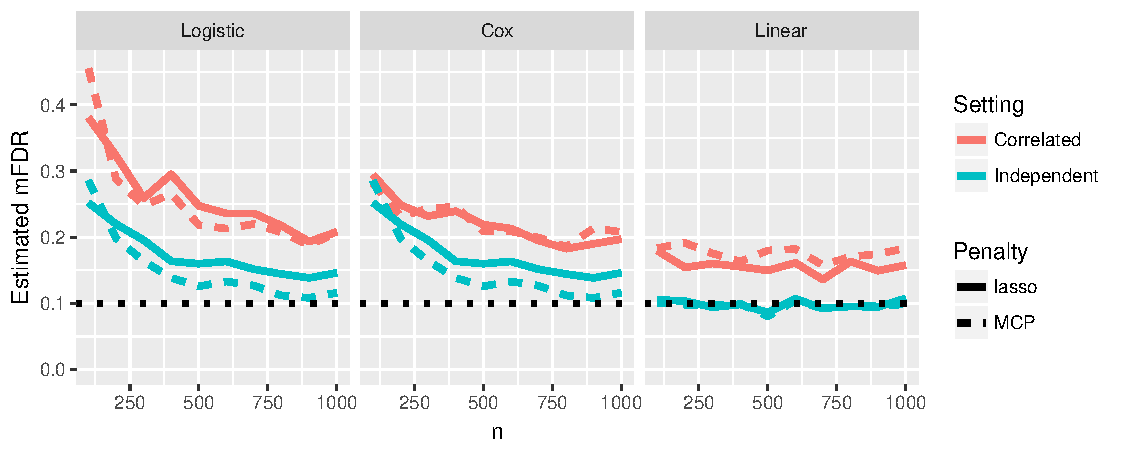
\includegraphics[width=.9\textwidth]{ggconverge3.pdf}
  \caption{Inaccuracy of the mFDR estimator}
\end{figure}

The mFDR estimator tends to be conservative, in the sense that the estimated false discovery rate is higher than the true FDR, with the degree of conservatism decreasing as $n$ increases. In the case of independent noise variables the estimator approaches the nominal marginal false discovery rate as $n$ increases. The convergence occurs nearly instantaneously for linear regression, with the estimator being very accurate even at $n=100$, and more slowly for logistic and Cox regression with the estimator remaining very slightly conservative even when $n > 500$. The MCP penalty leads to faster convergence and better accuracy than the lasso penalty; this is particularly noticeable in the logistic and Cox regression settings.

%% NOTE: This is discussed in ``Other Penalty Functions'' now
%% The improvement is likely due to the MCP's tendency towards less biased coefficient estimates which results in more accurate estimates of $v_j$ and also faster convergence of the remainder term.

The correlated setting induces a noticeable conservative bias that is cannot be resolved by increasing the sample size. This issue is not unique to mFDR as many methods for controlling false discovery rates also tend to be conservative in correlated settings.  Generally speaking, this conservative nature is not viewed as a significant drawback to false discovery rates, as it still allows one to control the fraction of false discoveries.  Furthermore, in this case, the effect is relatively slight: the estimated mFDR is many cases is around 20\% in cases where the true mFDR is 10\%, but nevertheless clearly identifies the values of $\lam$ for which the mFDR is low, and where it is high.

\subsection{Features associated with censoring}

As discussed in Section~\ref{Sec:cox}, the presence of censoring in Cox regression means that, strictly speaking, for Theorem~\ref{Thm:main} to apply, noise features cannot be associated with the censoring mechanism either.  Here, we assess the robustness of the mFDR estimator when this condition is violated.

\begin{table}[b!]
 \caption{Average true mFDR (10,000 simulations) when the estimated mFDR is 10\%}
\centering
\begin{tabular}{c | c c}
  \hline
 Scenario & lasso & MCP   \\  [0.5ex]
  \hline 
   A & 1.02\% & 6.72\% \\ 
   B &  1.33\% & 7.31\% \\ 
   \hline
\end{tabular}
\end{table}

Consider two scenarios, A and B. In each scenario censoring times are generated from exponential distributions with $\theta_{i} = \exp(\x_i^T \bg)$, and in scenario A four noise variables are related to censoring via
\as{\bg_A &= (0, 0, 0, 0, 1, -1, 1, -1, 0, \ldots, 0),}
while in scenario B all variables are independent of censoring with $\bg_B = \zero$.  By design, each of these scenarios, on average, results in 50\% of the observations being censored.  The same set of $n = 100$ true failure times is used for both scenarios and are generated from independent exponential distributions with rate parameter $\theta_i = \exp(\x_i^T \bb)$, where $\beta_{1:4} = 1$ and $\beta_{5:40} = 0$.

In scenario A, the association with censoring induces correlation between the noise features and leads to a slightly more conservative mFDR estimator. The degree of conservatism is quite minor, however, in comparison to the effects of sample size and correlation between noise variables studied in Section~\ref{Sec:accuracy}.

\subsection{Comparison with other methods}
\label{Sec:sim-comp}

In this section, we compare our proposed mFDR approach with other methods of variable selection used in the high-dimensional setting. We generate our data based upon the structure depicted in Figure~\ref{Fig:diagram}, using $n = 400$ and $p = 1000$ with ten variables are causally related to the outcome, like ``A'', such that $\beta_{1:10} = b$ and vary $b$ throughout the study. Corresponding to each causal variable we generate nine correlated ($\rho = 0.5$) variables, akin to ``B''. The remaining 900 variables are noise, akin to ``C'', however they are correlated with each other such that $Cor(\x_j,\x_k) = 0.8^{|j - k|}$, thereby creating a situation where the mFDR estimator will be conservative.

%% NOTE: Should the x-axis label here be ``b''? -- fixed

\begin{figure} [b!]
 \centering
  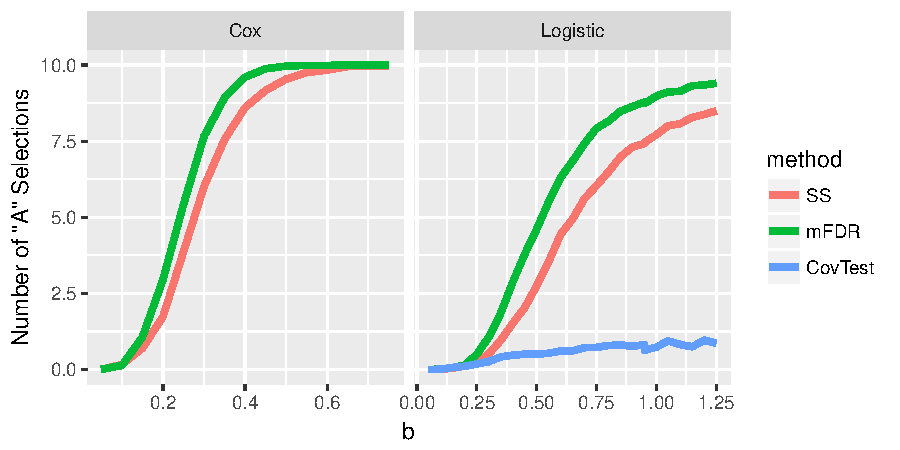
\includegraphics[width=0.75\textwidth]{ggpower.pdf}
  \caption{\label{Fig:lassopower} The number of true, ``A", variables selected by each lasso based method of false discovery rate control, averaged across 1,000 simulation iterations plotted as a function of $\beta$.}
\end{figure}

We assess the average number of selections for each variable type (``A'', ``B'', ``C'') after applying each of the following methods:
\begin{itemize}
\item Our mFDR approach, where variables are selected by the lasso using the smallest $\lambda$ with $\widehat{mFDR} \leq .1$.
\item A sample splitting approach, motivated by \citet{Sample_Splitting}, where we first fit a lasso regression model on half of the data to select the top 20 variables. We then use the remaining data to fit a unpenalized regression model on the variables selected in the first stage. With the unpenalized model we conduct traditional hypothesis tests on the regression coefficients and apply the Benjamini-Hochberg procedure \citep{BH_1995} to control the false discovery rate at $10\%$. Here, we limit the first-stage selections to 20 variables so that in the second stage, the model contains 10 events per variable \citep{peduzzi_epv}.
\item The covariance testing approach \citep{CovTest}, which we use in conjunction with the forward stopping rules proposed by \citet{GSell2016} to control the pathwise false discovery rate at $10\%$. 
\item A large scale univariate testing approach which fits an unpenalized regression model to each variable individually, conducts a hypothesis test on the variable coefficient, and then adjusts the resulting p-values using the Benjamini-Hochberg procedure to control the false discovery rate at $10\%$.
\item A lasso approach which uses 10-fold cross validation (CV) to select the $\lambda$ and makes no attempt to control the false discovery rate.
\end{itemize}

The results of this simulation are shown in Figure~\ref{Fig:lassopower}.  Compared to other false discovery rate control methods for penalized regression, the mFDR approach selects more causally important variables at every value of $b$. The covariance testing approach in particular selects far fewer causal features in the logistic regression setting than either mFDR or sample splitting, although it should be noted that despite being available in the {\tt CovTest} R package, the covariance test for logistic regression is currently considered to be experimental by the package creators.  The covariance test is not shown for Cox regression as this has not yet been implemented in the package.

%% NOTE: Change var to Type -- fixed

\begin{figure} [!htb]
 \centering
  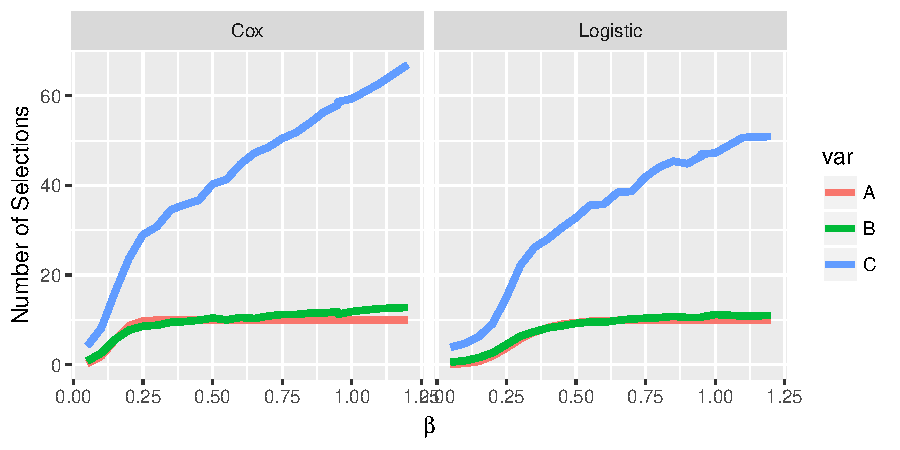
\includegraphics[width=0.75\textwidth]{ggcv.pdf}
  \caption{\label{Fig:cv} The average number of selections for each type of variable depicted in Figure~\ref{Fig:diagram} is plotted for cross validation as function of $\beta$.}
\end{figure}

%% NOTE: Clarification here, 80%, 10% -- how are B variables being counted? -- Considering B vars are valid selections, changed text to 75% (~60 C sels/~80 total sels)

Simulation results for cross validation are shown in Figure~\ref{Fig:cv}.  As the figure shows, while cross-validation tends to select nearly all the ``A'' variables, it does not control number of false selections.  In fact, it selects an increasingly large number of noise variables as the signal strength $b$ increases. Whereas sample splitting, covariance testing, and mFDR all resulted in false discovery rates well under 10\% throughout our simulations, as many as $75\%$ of the selections made by cross validation were noise variables for larger values of $\beta$.

%% NOTE: I don't understand what this sentence means...maybe let's talk about it and then we can reword and put it back in.  --- Keeping out for now
%% This is particularly troublesome since these additional noise variable selections offer no advantage when it comes to selecting true variables in this scenario, thus highlighting a major difference between using the lasso for prediction and using the lasso for variable selection.

\begin{figure} [!htb]
 \centering
  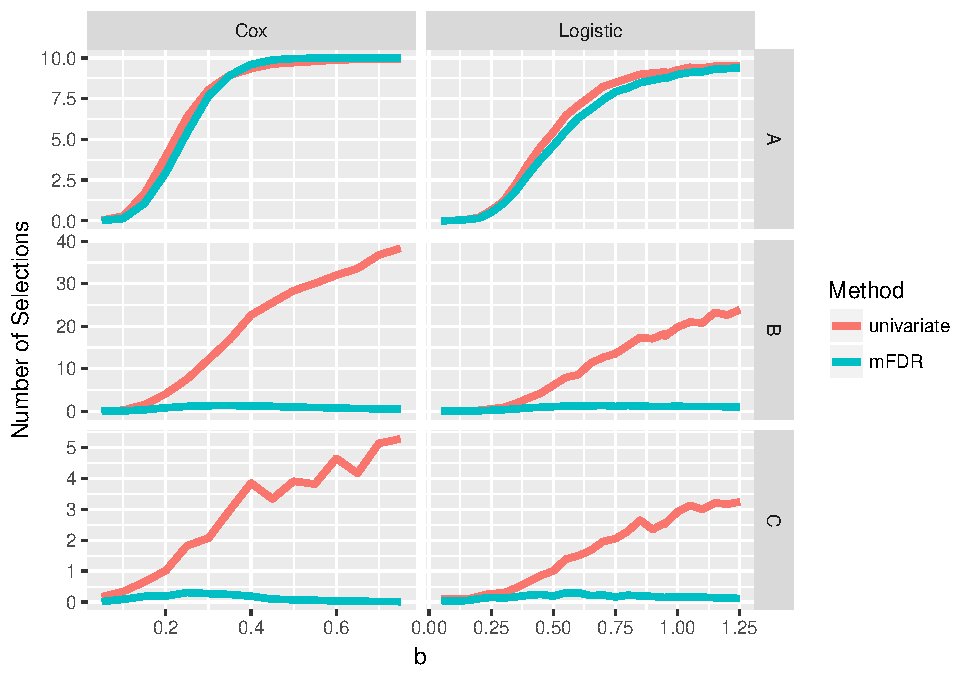
\includegraphics[width=0.8\textwidth]{ggunivariate2.pdf}
  \caption{\label{Fig:univariate} The average number of selections, for each type of variable depicted in Figure~\ref{Fig:diagram}, is plotted as function of $\beta$ for each method which controls the false discovery rate.}
\end{figure}

Figure~\ref{Fig:univariate} compares the mFDR and univariate approaches, both of which are designed to control the proportion of marginal false discoveries without making any claims pertaining to correlated, ``B'', variables. The top panels show that the two methods are comparable in terms of their ability to select the true causal variables.  The advantage of using a regression-based approach over univariate testing, however, is clearly seen when looking at the number of other selections.  Lasso with mFDR control greatly reduces the number of correlated (``B'') selections compared to univariate testing: whereas univariate testing tends to identify dozens of indirectly associated features as discoveries, lasso with mFDR control tends to select at most two.

%% NOTE: Leftover from a previous version of this figure? -- yes, can be removed
%% The mFDR approach even does as well at limiting correlated variable selections as the sample splitting and covariance approaches which are based upon fully conditional and pathwise conditional false discovery definitions respectively, all three of these approaches make nearly zero correlated variable selections for all values of $\beta$.

In Figure~\ref{Fig:univariate}, mFDR also selects far fewer noise (``C'') variables than univariate testing.  The reason for this is that the large number of ``B'' features selected by univariate testing allows it to select many more ``A'' and ``C'' features while maintaining the overall FDR at a level less than 10\%.  For this reason, Figure~\ref{Fig:univariate} is potentially somewhat misleading in terms of comparing mFDR and univariate testing in terms of their power to identify type ``A'' features.

Table~\ref{Tab:univariate} presents an alternative metric for comparing the univariate and mFDR approaches.  Given the overwhelming difference between the two approaches with respect to type ``B'' features, the table presents the ratio of the number of causally associated features to the number of noise features -- i.e., the A:C ratio -- for various values of $\beta$.  Whereas Figure~\ref{Fig:univariate} indicated that the two approaches were approximately equally effective at identifying the truly important variables, Table~\ref{Tab:univariate} shows that the lasso-mFDR approach was far more powerful as measured by comparing the number of true discoveries to the number of false discoveries.

\begin{table}[b!]
\centering
\begin{tabular}{c | r r r r}
  \hline
  & \multicolumn{2}{c}{Cox} & \multicolumn{2}{c}{Logistic}\\
 $\beta$ & Univariate & Lasso-mFDR & Univariate & Lasso-mFDR \\ 
  \hline
  0.25 & 3.5 & 17.7 & 2.3 & 3.3 \\ 
  0.35 & 3.0 & 36.2 & 4.9 & 11.1 \\ 
  0.45 & 2.9 & 102.2 & 5.3 & 15.3 \\ 
  0.65 & 2.4 & 333.3 & 4.6 & 32.6 \\ 
  0.75 & 1.9 & 750.0 & 4.1 & 47.6 \\ 
   \hline
\end{tabular}
\caption{\label{Tab:univariate} The ratio of A:C variable selections for various values of $\beta$.}
\end{table}

Indeed, for the univariate approach, the rate of true variable selections per noise variable selection is not only low, but in fact decreases as $\beta$ increases. In contrast, with the mFDR approach, the true variable to noise variable selection rate increases with $\beta$ as one would hope.

\section{Case studies}

\subsection{Lung cancer survival and gene expression}

\citet{Shedden2008} studied the survival of 442 early-stage lung cancer subjects. Researchers collected high-dimensional gene expression data consisting of 22,283 genes and additional clinical covariates of age, race, gender, smoking history, cancer grade, and whether or not the subject received adjuvent chemotherapy.

\textcolor{red}{NOTE: Add more on outcome: is the outcome time to death?  From when?  How many events?}

In our analysis we aim to select important genes while controlling the marginal false discovery rate.  We use a penalized Cox proportional hazards regression model that allows for all of the clinical covariates to enter the model unpenalized while using the sparsity introduced by penalization to screen for additional genes related to survival.  We target an mFDR of 10\% and compare our results to those of other methods.

\begin{figure} [!htb]
 \centering
  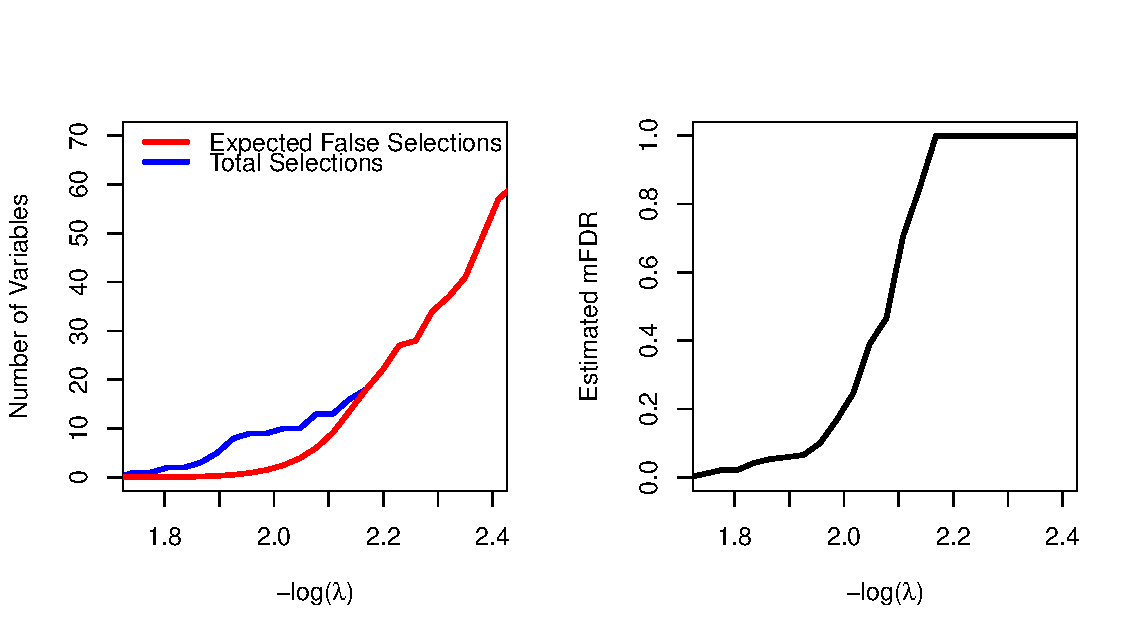
\includegraphics[width=0.65\textwidth]{Shedden.pdf}
  \caption{\label{Fig:Shedden} False discovery estimates for the Shedden data at each value of $\lam$.  (left) total number of features selected and expected number of false discoveries; (right) estimated mFDR.}
\end{figure}

Figure~\ref{Fig:Shedden} illustrates the false discovery rate estimates for this study.  On the left, we see a gap between the number of selections and the expected number of false selections for many values of $\lambda$.  This indicates that for these values of $\lam$, many of the genes selected by the lasso are likely to be truly related to survival, as it would be unlikely for so many noise features to selected merely by random chance.

\textcolor{red}{This has to be a mistake, right?}

\begin{table}[htb!]
\centering
\begin{tabular}{c | r r r r r }
  \hline
lasso & $\lambda$ & EF & S & mFDR & cross validation error \\ 
	\hline
	CV & 0.1215 & 9.16 & 13 & 70.4\% &  1307.9 \\
	CV(1se) & 0.180  &  0 &  0 &  -  & 1320.2 \\
	mFDR & 0.146 & 0.52 & 8 & \textcolor{red}{0.07\%} & 1313.3 \\
\hline
MCP & $\lambda$ & EF & S & mFDR  & CV error \\
	\hline
	CV & 0.1331 & 2.53 & 8 & 31.7\% &  1309.7 \\
	CV(1se) & 0.180 & 0 & 0 & - &  1320.4 \\
	mFDR & 0.155 & 0.16 & 2 & 8.2\% &  1315.1 \\
		\hline
\end{tabular}
\caption{\label{Tab:shedden} Results comparing different $\lambda$ choices, along the default sequence generated by {\tt ncvreg}, using the lasso and MCP penalties on the Shedden data }
\end{table}

Table~\ref{Tab:shedden} displays results for three potential approaches to choosing $\lam$: the value that minimizes cross-validation error (CV), the value that comes within 1 standard error of minimizing CV (1se) \textcolor{red}{Maybe a citation here?}, and the smallest value of $\lam$ satisfying $\mFDR < 10\%$.  The uniform shrinkage applied by the lasso inherently creates a tradeoff between optimal prediction and accurate variable selection. In this case, we see that the lasso model with lowest prediction error has an estimated mFDR of 70.4\%, indicating that despite its prediction accuracy, a substantial fraction of the 13 features selected by the model may be noise. Conversely, if we aim to control the mFDR at 10\%, we select only 8 features.  Although we can be more confident that these 8 features are truly related to survival, the model is somewhat less accurate from a prediction standpoint (CV error of 1313 compared to 1308).  An alternative suggested in the popular text \textit{The Elements of Statistical Learning} is to select the largest $\lambda$ whose CV error is within one standard error of the minimum, a choice we refer to by CV(1se), with the idea being that this choice results in a more parsimonious model whose accuracy is comparable with the best model \citep{Hastie2009}.  In this example the CV(1se) results in the null model, an undesirable result from a feature selection perspective.  However this result suggests that mFDR model, which selects 8 features with confidence, also has accuracy that is comparable with the best model.  

%\textcolor{red}{Something about the 1se approach.}

An alternative to lasso-penalized regression is to use the MCP penalty, which relaxes the degree of shrinkage for large coefficients, thereby allowing a smaller number of features to account for the observed signal.  The MCP model that minimized CV error had an estimated mFDR of only 31.7\%; compared to the lasso model that minimized CV error, we can be considerably more confident in the smaller number of features selected by MCP.  The prediction accuracy of MCP was similar to lasso in this case (CV error 1310 vs. 1308), with the lasso being slightly more accurate and MCP slightly more parsimonious.

MCP strikes an attractive balance in this case between prediction accuracy and false discovery rate.  One reason for this is that two genes, 205308\_at, and 221249\_s\_at \textcolor{red}{(Gene names would be better than these codes)}, have very large effects, exactly the scenario MCP is designed to perform well in. In the lasso model with $\lambda$ selected by cross validation these variables have coefficients of -0.170 and -0.118 respectively, while in the MCP model these variables have coefficients of -0.220, -0.175 despite cross-validation selecting a larger $\lambda$ for MCP.  Again, this illustrates the fact that lasso models can only accommodate large effects by lowering $\lambda$, which comes at the cost of allowing additional noise variables into the model.

For comparison we also analyzed the data using repeated sample splitting with 100 random splits, as advocated by  \citet{Meinshausen2009}. However, this approach was unable to select any genes at a false discover rate \textcolor{red}{of 10\%?  20\%?  It would be nice to say something here like, even if we went to 50\%, it still couldn't select anything}.  As mentioned earlier, the {\tt covTest} package does not (currently) accommodate survival data.

We also applied a large scale univariate testing approach to the Shedden data, fitting a series of Cox regression models adjusting for all clinical covariates and containing a single gene.  After using the Benjamini-Hochberg procedure to control the false discovery rate at 10\%, this approaches selects 803 genes, far more than any of the regression-based approaches.  As discussed in Section~\ref{Sec:sim-comp}, the primary difference between univariate and regression-based methods with respect to false discoveries is that univariate approaches tend to select large numbers of features that are indirectly correlated with the outcome.  Our simulation results would suggest that for these data, univariate testing yields a large number of genes, most of which are only indirectly associated with survival, while the mFDR approach yields a smaller number of genes, most of which are directly associated with survival.

\subsection{Lung cancer status among smokers}

\citet{Spira2007} collected RNA expression data from histologically normal bronchial epitheliums of $n = 192$ smokers of which 102 had developed lung cancer and 90 had not developed lung cancer.  We are interested identifying genes that are indicative of whether or not a smoker has lung cancer.  For our analysis we fit a penalized logistic regression model using both the lasso and MCP penalties. We compare the results at $\lambda$ values chosen using estimated mFDR, cross validation, and the covariance test as well as the selections made by sample splitting. We also compare these model-based approaches to the traditional univariate approach with false discovery rate control.

% NOTE: Should this table go out further, to show CV lambda?

\begin{table}[htb!]
\centering
\begin{tabular}{c | r r r r r r }
  \hline
lasso & $\lambda$ & EF & S & mFDR & misclassification error & cross validation error \\ 
	\hline
	CV & 0.0294 & 49 & 49 & 100\% & 24.5\% & 0.995 \\
	CV(1se) & 0.0627 & 32 & 32 & 100\% & 25.0\% & 1.074 \\
	mFDR & 0.146 & 0.785 & 10 & 7.8\% &  30.7\% & 1.289 \\
\hline
MCP & $\lambda$ & EF & S & mFDR & misclassification error & cross validation error \\
	\hline
	CV & 0.0775 & 13 & 13 & 100\% & 30.2\% & 1.113 \\
	CV(1se) & 0.0929 & 10 & 10 & 100\% & 33.3\% & 1.182 \\
	mFDR & 0.1508 & 0.42 & 5 & 8.4\% &  33.9\% & 1.306 \\
		\hline
\end{tabular}
\caption{\label{Tab:spira} Results comparing different $\lambda$ choices using the lasso and MCP penalties on the Spira data }
\end{table}

Table~\ref{Tab:spira} shows results for various $\lambda$ values and penalty functions applied to the Spira data.  In contrast with the Shedden case study, in this example cross validation selects a $\lambda$ value corresponding to an estimated mFDR of 100\% for both the lasso and MCP penalties.  As discussed throughout the paper, this should be taken more as an upper limit than as an unbiased estimate, but the overall implication is that it is easy for many noise variables to enter these models by chance along and we should be cautious about making conclusions concerning variables selected by cross validation.

%% Table~\ref{Tab:spira} presents estimated marginal false discovery rates for various values of $\lam$ near 10\%.  The largest number of genes we can select without exceeding a 10\% mFDR is ten, and occurs at $\lam=0.1463$.  Cross validation selects a $\lambda$ of 0.056; although not shown on this table, the estimated number of false discoveries at that value of $\lam$ exceeds the number of selected genes, resulting in an estimated mFDR of 100\%.  As discussed throughout the paper, this number should be taken more as an upper limit than an unbiased estimate, but the overall implication is clear: at $\lam=0.056$, it is very easy for noise features to enter a lasso model by chance alone, so one should be very cautious about drawing conclusions concerning the variables selected by cross-validation, as false discoveries are likely abundant.

%% NOTE: IS THIS CONSISTENTLY THE CASE?  IF YOU RUN CROSS VALIDATION A FEW TIMES, DO YOU EVER GET SOMETHING CLOSER LIKE, SAY, 9 GENES OR SOMETHING?

%% Using the MCP penalty instead of the lasso for this data, at a 10\% mFDR we select a $\lambda$ value of 0.1508, corresponding to 5 genes.  Using cross validation, 14 genes are selected, although the estimated mFDR is again 100\%. The comments regarding mFDR and cross validation in the previous paragraph apply to MCP as well, although the disparity between the mFDR model and CV model is smaller than for the lasso.

We also analyzed this data using the sample splitting and covariance testing approaches.  The sample splitting approach, using 100 random splits, does not select any features after controlling the false discovery rate. Only a single gene reached the second stage in at at least half of the splits but its median p-value was not significant. Similarly the covariance testing approach also does not select any features.  The first variable to enter the model has a p-value of 0.475 and when the ForwardStop procedure is applied we are unable to move beyond the intercept only model without the false discovery rate exceeding 10\%.

Finally, we applied the univariate testing approach to these data in two ways. First, we used t-tests to assess the difference in expression for each gene for the two groups while controlling the false discovery rate at 10\% using the Benjamini-Hochberg procedure.  This procedure selects selecting 2,965 genes. Second, we fit a series of univariate logistic regression models; using this approach selects 2,833 genes at a 10\% mFDR. Once again, depending on the goals of the analysis and whether indirect associations are of interest, either the univariate or mFDR approach might prove useful here.  However, fully conditional and pathwise conditional approaches to controlling the false discovery rate tend to too restrictive to actually identify any features in many real high-dimensional studies.

\section{Discussion}

Estimating the marginal false discovery rate of a penalized likelihood model is a useful way of assessing the reliability of a selected set of features. Unlike other approaches that have a similar goal, such as sample splitting or the covariance test, mFDR uses less strict definition of a false discovery which does not require conditioning on any other variables and consequently only limits the selection of variables that are noise in an unconditional -- i.e., marginal -- sense.  The simulation comparisons in this paper demonstrate that while mFDR is based upon a weaker false discovery definition, it can do quite well in limiting the number of correlated, non-causal variable selections.

The mFDR estimator is currently implemented in R in the {\tt ncvreg} package \citep{Breheny2011} using the {\tt mFDR} function. The function accepts an ncvreg fitted model and provides estimates for the expected number of false discoveries, as well as the mFDR for each value of the $\lambda$ sequence used in fitting the model.  These are obtained by calling {\tt mFDR(fit)}; the package also provides a plotting method, which produces plots like those in Figure~\ref{Fig:Shedden}.  The {\tt ncvreg} package accommodates lasso, MCP, SCAD, elastic net, and MNet \citep{Huang2016} penalties and provides a convenient model summary measure for penalized regression models.

%% NOTE: Would be nice to mention time here (or in previous section): How long do each of these methods take to run?  -- added table and paragraph below
\begin{table}[ht]
 \caption{\label{Tab:time} The elapsed time, in seconds, of each approach in each of our case study analyses.}
\centering
\begin{tabular}{rrrrr}
  \hline
 & mFDR & Sample Splitting & CovTest & Univariate Testing \\ 
  \hline
	Shedden & 7.0 & 1882.9 & NA & 232.1 \\
Spira & 1.4 & 568.1 & 571.1 & 41.0 \\ 
   \hline
\end{tabular}
\end{table}

Table~\ref{Tab:time} displays the run time of each analysis approach used on the case study data of Section 4. For the Spira data, where $n = 192$ and $p =22215$, using {\tt ncvreg} to fit a penalized logistic regression model and then estimating the mFDR for the entire $\lam$ sequence takes only 1.4 seconds. This is nearly 30 times faster than univariate testing, and over 400 times faster than the model based approaches, sample splitting and CovTest.  Similar results are seen for the Shedden survival data.  The speed at which mFDR can be calculated makes it a useful addition to any penalized regression analysis.

This manuscript has demonstrated how to extend control over the marginal false discovery rate for penalized regression models to any general likelihood-based loss function.  The method is shown to be more powerful than competing approaches and currently offers better software support.  Estimation of the marginal false discovery rate for penalized likelihood models is a fast, convenient, easily interpreted, and broadly useful approach to inference concerning the reliability of feature selection, and is capable of being generalized to a wide variety of penalty functions and regression modeling frameworks.
